\chapter{\label{ch:x-misc}Miscellaneous notes}

\minitoc

\section{To do}

\begin{enumerate}
	\item HYADES simulations
	\item Add more citations
	\item Similarity theory details in appendix
	\item Add details on CPA and OPCPA
	\item Simulation algorithms (details in appendix?)
	\item Velocity transformations derivation (appendix)
	\item Sources of error system
	\item Ponderomotive heating mechanisms
	\item Fix QED section
	\item Particle merging
	\item Radiating particles and relativistic larmor radius
	\item smieli performance plot
	\item A collisionless fully ionised plasma
	\item Basic derivation of the Schwinger limit
	\item Calculating collision frequency
	\item Feynmann diagrams
	\item Add some detail of vectorisation
\end{enumerate}

On the ZVP front
\begin{enumerate}
	\item Fix diagrams
	\item Go through discussions
	\item Add errrors plot
	\item Check out new sims
	\item Conclusion
	\item Shape of transverse momentum (more parabolic compared to linear and explanaition of bunch holding together), Shrp front edge then parabolic (or even exponential decay - it is defo expoenential)
	\item a0 convention, when max and when varying in time
	\item Editing
\end{enumerate}

\section{ORION experiment} 
The following derivation determines the polarisation of the ORION laser pulses in the experiment and the boostes frame quantities for the PIC simulations.

I will have a whole subsection devoted to the different frames of reference of relevance and then a second one about normalised units. What follows now is the derivation of the boosted frame in which the laser is incident normally relative to the lab frame where the laser is incident obliquely.

I will try to use a consistent convention for coordinate system as much as possible.

\subsection{Frames of reference}
Other frames of reference include, HB front surface at rest frame, ablating front frame, smilei frames. 

When writing out the pistoning equation in full in thesis, include analysis in Robinson 2009 to do it for multiple ion species.



I should go over this and use third year relativity notes to formalised and make more consistent.

While some of this section may seem trivial, it is frequently miscalculated in the literature, it therefore seems of great importance to provide a full derivation.

The following is inspired by \cite{bourdierObliqueIncidenceStrong1983}, here they give the formula for k and omega.

In \cite{bourdierDynamicsChargedParticle2001} they determine the normalised vector potential, if defined similarly in the new frame, then it is frame invariant. This fails to consider what about the fact that the vector potential is in reality more complex and is not simply the temporal integral of the electric field. Nonetheless it is still reasonable to define it so if what is of real importance (as is usually important) is in fact the fields and it is simply being used as a way to normalise the field intensity.

Consider a photon incident on a plasma block at angle $\theta$ as in figure \ref{fig:miscreferenceframesboosted1d}.
% TODO: \usepackage{graphicx} required
\begin{figure}
	\centering
	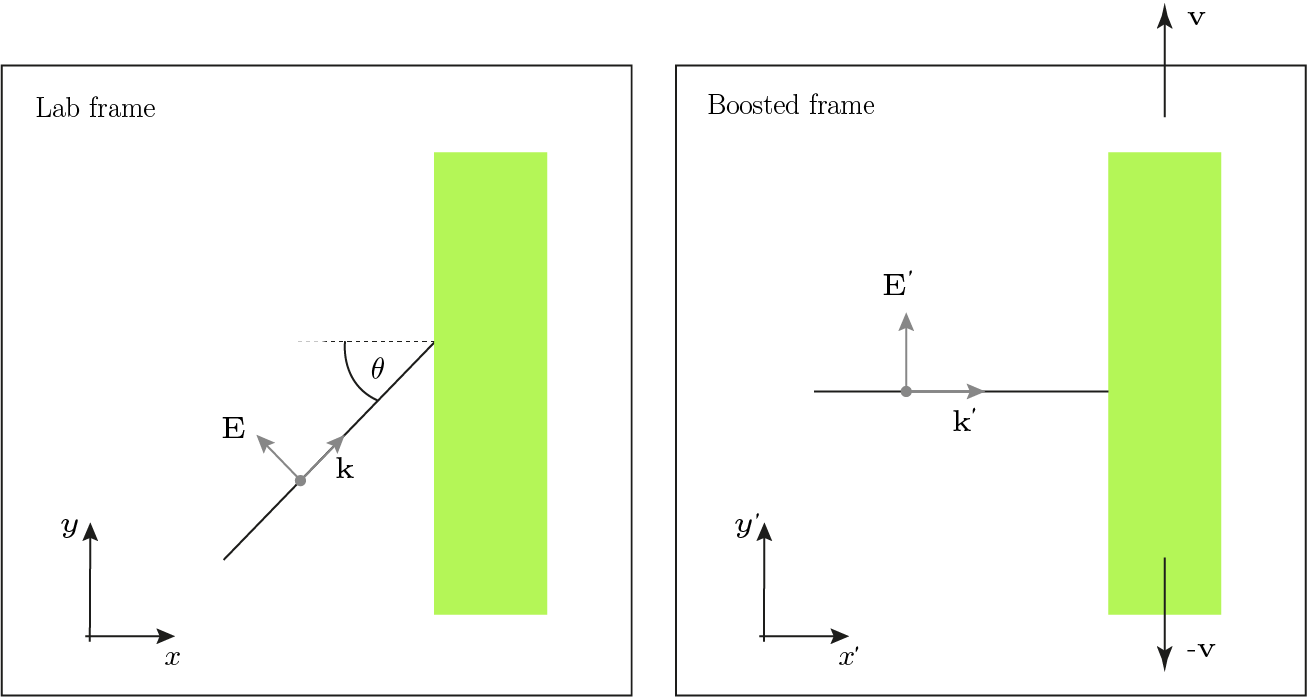
\includegraphics[width=1\linewidth]{figures/misc/misc_reference_frames_boosted_1D}
	\caption{}
	\label{fig:miscreferenceframesboosted1d}
\end{figure}
A boost is applied with velocity $\mathbf{v}$ to a frame such that the photon is normally incident on the now streaming plasma at velocity $-\mathbf{v}$. The velocity transformation for the photon's velocity, $\mathbf{u}$, parallel to the boost is
\begin{equation}
	\mathbf{u}'_\parallel = \frac{\mathbf{u}_\parallel - \mathbf{v}}{1-\mathbf{u}\cdot\mathbf{v}/c^2}.
\end{equation}
Setting  $\mathbf{u}'_\parallel = 0$, it is clear that
\begin{equation}
	\mathbf{v} = \mathbf{u}_\parallel = c\sin\theta \hat{\mathbf{y}}
\end{equation}
in this geometry and 
\begin{equation}
	\gamma_\mathbf{v} = \frac{1}{\sqrt{1-\mathbf{v}^2/c^2}}=\sec\theta.
\end{equation}
Noting that since Snell's law is frame invariant, the photon remains normal as it propagates into the skin depth of the plasma, a frame in which the interaction reduces to a 1D problem has been successfully found for all $\theta < \pi/2$. Those familiar with the topic may wonder how this is possible considering the `ripples' that are observed on the plasma surface for oblique incidence. The explanation for this is of course the relativity of simultaneity. It remains to determine how do all the relevant quantities transform as such a boost is applied. Starting with an easy one: the photon's wave four-vector is 
\begin{equation}
	\mathbf{K}^\mathrm{\mu} = \left(\frac{\omega}{c},\mathbf{k}\right)
\end{equation}
and thus the freqency transforms as
\begin{equation}
	\frac{\omega}{c} = \gamma_\mathbf{v}\left(\frac{\omega'}{c}-\frac{\mathbf{v}}{c}\cdot\mathbf{k'}\right).
\end{equation}
Since $\mathbf{v}\cdot\mathbf{k'} = 0$, 
\begin{equation}\label{eq:boost_omega}
	\omega' = \omega\cos\theta .
\end{equation}
As 
\begin{equation}
	n'_\mathrm{c} = \frac{m_\mathrm{e}(\omega')^2}{4\pi e^2},
\end{equation}
\begin{equation}\label{eq:boost_nc}
	n'_\mathrm{c} =n_\mathrm{c} \cos^2\theta ,
\end{equation}
while the plasma block will be Lorentz contracted along $\hat{\mathbf{y}}$, hence the number density of electrons will increase as,
\begin{equation}
	n'_\mathrm{e} = \frac{n'_\mathrm{e}}{\cos\theta},
\end{equation}
leading to the perhaps unexpected
\begin{equation}
	\bar{n}'_\mathrm{e} = \frac{\bar{n}_\mathrm{e}}{\cos^3\theta}.
\end{equation}
Time is dilated 
\begin{equation}
	t' = \frac{t}{\cos\theta}.
\end{equation}

Consider now the more general case (I should jsut simply replace my diagram with a 3D one that incorporates this initially) where the photon's electric field is rotated out of the $x$-$y$ plane, \textit{i.e.}
\begin{equation}
	\mathbf{E} = E_0(-\cos\phi\sin\theta,\cos\phi\cos\theta,\sin\phi)
\end{equation}
and correspondingly
\begin{equation}
	\mathbf{B} = \frac{\hat{\mathbf{k}} \times \mathbf{E}}{c}= \frac{E_0}{c}(\sin\phi\sin\theta,-\sin\phi\cos\theta,\cos\phi).
\end{equation}
The Lorentz transformations for electro-magnetic fields are
\begin{equation}
	\mathbf{E}'_\parallel = \mathbf{E}_\parallel,
\end{equation}
\begin{equation}
	\mathbf{B}'_\parallel = \mathbf{B}_\parallel,
\end{equation}
\begin{equation}
	\mathbf{E}'_\perp = \gamma_\mathbf{v}(\mathbf{E}_\perp + \mathbf{v} \times \mathbf{B}),
\end{equation}
\begin{equation}
	\mathbf{B}'_\perp = \gamma_\mathbf{v}(\mathbf{B}_\perp - \mathbf{v} \times \mathbf{E}/c^2).
\end{equation}
Using the above expressions for $\mathbf{E}_\perp$ and $\mathbf{E}_\parallel$ and transforming to the boosted frame,
\begin{equation}
	\mathbf{E}' = E_0\cos\theta (0,\cos\phi,\sin\phi).
\end{equation}
As anticipated for normal incidence there is no component of the E-field normal to the surface. Conveniently, the polarisation of the incident photon is unchanged despite having components both parallel and perpendicular to the transformation and 
\begin{equation}
	|\mathbf{E}'| = |\mathbf{E}|\cos\theta.
\end{equation}
The picture can now be completed. Since
\begin{equation}
	a_0' = \frac{e|\mathbf{E}'|}{m_\mathrm{e}e\omega'}
\end{equation}
it follows that
\begin{equation}
	a_0' = a_0,
\end{equation}
\begin{equation}
	S' = \frac{S}{\cos^3\theta}.
\end{equation}


\subsubsection{Four-potential transformation}
Consider a laser pulse obliquely incident, angle $\theta$, it has 4-vector potential $\mathbf{A}^\mu = (0, A\sin\theta,A\cos\theta,0)$, where $A = A_0\sin(\mathbf{k}\cdot\mathbf{x} - \omega t)$ and $\mathbf{k} = (k\cos\theta,k\sin\theta,0)$. Applying the lorentz transformation, in the frame where the laser pulse is normally incident,
\begin{equation}
	\mathbf{A}'^\mu = (-\gamma\beta A\cos\theta/c,  - A\sin\theta, \gamma A\cos\theta,0) = (-A\sin\theta, -A\sin\theta, A,0) 
\end{equation}
since $\beta = \sin\theta$ in the positive $y$ direction and $\gamma = 1/\cos\theta$.

Therefore,
\begin{equation}
	\mathbf{E}'/\cos(\mathbf{k}\cdot\mathbf{x} - \omega t) = --\sin\theta\cos\theta k A_0\hat{\mathbf{x}} --- \sin\theta\cos\theta \omega A_0\hat{\mathbf{x}} + A_0\omega\cos\theta = A_0\omega',
\end{equation}
since $\sin(\mathbf{k}\cdot\mathbf{x} - \omega t) = \sin(x'k\cos\theta-\omega t'\cos\theta)$
Note I have been sloppy here with factors of $c$.

Do it does look at though the vector potential amplitude is unchanged by the transformation but it is more subtle, it is useful to define an $a_0' = eE/m_\mathrm{e}\omega$ to normalise the electric field intensity but note that this cannot be converted into the actual vector potential, it is just a useful construct.

Also note that whatever the transverse vector potential is in the boosted normal incidence frame is simply whatever the amplitude of the vector potential is in the oblique incidence frame.

\subsection{ORION interaction geometry}
The ORION target chamber has its own defined geometry with the target located at the origin, described in figure \ref{fig:miscoriontargetchambergeometry}.
% TODO: \usepackage{graphicx} required
\begin{figure}
	\centering
	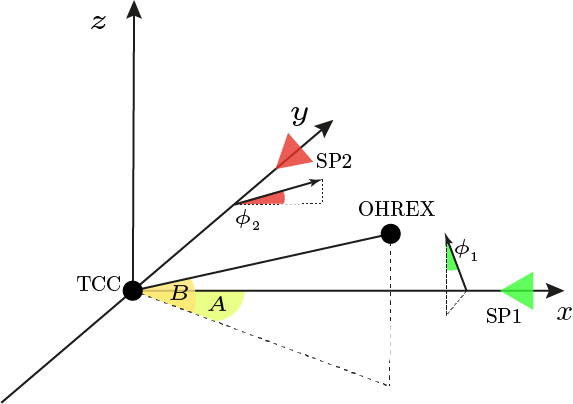
\includegraphics[width=0.5\linewidth]{figures/misc/misc_ORION_target_chamber_geometry}
	\caption{ORION target chamber geometry showing the location of the target (TCC) and OHREX spectrometer and the green (SP1) and infra-red (SP2) beamlines and their corresponding polarisations.}
	\label{fig:miscoriontargetchambergeometry}
\end{figure}
The polarisation angles are $\phi_1 = \qty{11.8}{\degree}$ and $\phi_2 = \qty{16.4}{\degree}$. Following reflection of the infra-red beam off the plasma mirror, both the green and infra-red lasers propagate in the -$\hat{\mathbf{x}}$-direction  towards the origin. The OHREX crystal is located at 
\begin{equation}
	\mathbf{r}_\mathrm{OHREX} = r_0(\cos B\cos A,-\cos B\sin A, \sin B),
\end{equation}
where $r_0 = \qty{2.4}{m}$, $A = \qty{26.82} {\degree} $ and $B = \qty{18.15}{\degree}$, setting the rotation angle of the target. This was achieved using the ORION Multi-Target-Mounts. Alignment was performed by Ed Gumbrell and no further details will be provided here on that process. 

The interaction plane is therefore defined by the vector
\begin{equation}
	\mathbf{n} = \frac{\mathbf{r}_\mathrm{OHREX}}{r_0} \times  \hat{\mathbf{x}} = (0,\sin B, \cos B\sin A).
\end{equation}
The cosine rule can be applied to determine the polarisation of the laser pulses in the interaction plane, for polarisation vector $\hat{\mathbf{E}}$,
\begin{equation}
	\frac{\mathbf{n}}{|\mathbf{n}|}\cdot\hat{\mathbf{E}} = \cos\theta,
\end{equation}
where $\theta$ defines the angle between the polarisation vector and the vector normal to the interaction plane. This corresponds to angles out of the interaction plane of 42.2 \degree for the SP1 beam (rotating anticlockwise out of the interaction plane when looking from TCC to parabola) and 19.6 \degree for the SP2 beam (rotating clockwise out of the interaction plane when looking from TCC to parabola). Again applying the cosine rule, the angle of incidence is 16\degree .


Next up: Polarisation on OHREX interaction plane.

The same method can be applied to determine the polarisation of the OHREX crystal interaction plane. The OHREX crystals have a nominal Bragg angle of 51.3\degree.

I still need to know the exact orientation of the OHREX but assuming it is vertical, the interaction plane is defined by
\begin{equation}
	\mathbf{n}_\mathrm{O} =  \frac{\mathbf{r}_\mathrm{OHREX}}{r_0} \times \hat{\mathbf{z}}= (-\sin A, -\cos A, 0),
\end{equation}
once it has been normalised.

Then again applying the cosine rule, this plane corresponds to angles out of the interaction plane of \qty{10.5}{\degree} for SP1 and \qty{58.9}{\degree} for SP2.

Is has been assumed that the non-linear RPM mechanism retains the polarisation of the incident laser pulse in the reflected harmonic beam.

Then since the OHREX crystal reflection is a linear process, we can decompose our incident beam into its polarisation constituents and consider what their combined intensity post reflection at the detector plane will be.

Also discuss the fabulous result that generally one can simply extract the results in the Smilei units and multiply by the relevant factors of the frame of interest and thus not worry too much about frame transformations.

Also check the boosted frame results against the bouchard thesis.


Once I have finished this section I must redo boosted section since I have made a mistake there and rethink a bit about optimum theta.

I must also at some point just state that a hat indicates a normalised vector.

%TODO Note that this section needs redoing, there is a new jupyter lab notebook for calculating values in ORION_analysis_sims/experiment_data_analysis on archer2 and called polarisations.ipynb


\subsection{Condition on validity of hole boring expression}
Robinson \textit{et al} \cite{robinsonHoleboringRadiationPressure2009} consider for what case is the expression they derive for hole boring valid. The case they are interested in is what happens if the energy available for an ion to gain from crossing the pseudo-capacitor is less than the kinetic energy associated with the hole boring velocity. Their analysis applies for non-relativistic hole boring velocities and circular polarised laser pulses. This theory is now updated for the ZVP mechanism (linear polarised and relativistic ion velocities).

The so-called `piston' which leads to ion hole boring is the pseudocapacitor field. In section \ref{sec:zvp_energies_derivation}, the development of that field is discussed quantitatively. The peak electric field is
\begin{equation}
	E_\mathrm{C} = E_\mathrm{L} = \sqrt{\frac{I}{\epsilon_0 c}}
\end{equation}
and the peak displacement of electrons is 
\begin{equation}
	\Delta x = \frac{\epsilon_0 E_\mathrm{C}}{en_\mathrm{e}}.
\end{equation}

Considering instead the relativistic kinetic energy gained by an ion were it to fully cross the pseudocapacitor, following equation \ref{eq:zvp_T},
\begin{equation}
	T_i = Z_i \times \frac{1}{2}m_\mathrm{e}c^2 \frac{a^2_0}{\bar{n}_\mathrm{e}} = \frac{IZ_i}{2cn_mathrm{e}}.
\end{equation}
(The equation above needs more thinking about)

Ions are reflected provided,
\begin{equation}
	T_i > \frac{1}{2}m_iv^2_\mathrm{HB}.
\end{equation}

Hmm ok so in Vincenti, they approximate electron mass as much less than ion mass and therefore neglect in the momentum calculation. It also looks like they have not done full relativistic calculation, so I cannot yet say I have that. But carrying on the derivation using Vincenti expression for simplicity:

The hole-boring velocity as calculated by Vincenti \textit{et al} \cite{vincentiOpticalPropertiesRelativistic2014} is
\begin{equation}
	\frac{v_\mathrm{HB} }{c}= \sqrt{\frac{R\cos\theta}{2}}
\end{equation}

So come back to this section, once I have fully written out the hole boring calcualtino in full, include also the multiple ion species stuff and this condition.

The upshot of this condition is something like: require no low charge to mass ratio ions (ie v heavy ions) and fully ionisation, these conditions are satisfied in this area of study.

To arrive at that result, useful parts include:
composite mass density $\rho = \sum_i m_i n_i$, $m_i = A_i/N_\mathrm{A}$ and $A_i \approx 2Z_i$ for most low mass ions relevant in these plasmas.




\section{Thinking about the ZVP calculation}
When I run sims on oblique incidence, this is another theorem that could be interesting to test.

Consider now that the surface moves inwards at speed $c$. In a time $\Delta t$, an energy $\sim B_\mathrm{L}^2\Delta t$ is incident on the surface. If at such a point, there exists a pseudocapacitor with electric field $E_\mathrm{C} \sim n_\mathrm{e}x_\mathrm{e}$, then the work done by pushing it inwards is $\sim E_\mathrm{C} n_\mathrm{e}x_\mathrm{e} \Delta x \ sim E_\mathrm{C}^2\Delta t$, since surface moving inwards at speed $c$. Thus by conservation of energy, the reflected field is $B_\mathrm{R}^2 = B_\mathrm{L}^2 - E_\mathrm{C}^2$. Note that at max displacement this cannot possibly be the case and we do see that the surface stops moving inwards, however this could be due to a reduction in the laser pulse intensity since the peak has passed. Thus this could be a reasonable approximation of the phenomena.

Then the force equilibrium expression in the boosted frame is
\begin{equation}
	-B_\mathrm{L} - \sqrt{B_\mathrm{L}^2 - E_\mathrm{C}^2} \pm B_\mathrm{i} + E_\mathrm{C}
\end{equation}
working this through one finds,
\begin{equation}
	x_\mathrm{p} = \frac{\cos^2\theta}{kS}\frac{2(1\pm \sin\theta)}{\sin^2\theta \pm 2\sin\theta +2}
\end{equation}
\begin{equation}
	T \sim \left(\frac{\cos^2\theta}{kS}\frac{2(1\pm \sin\theta)}{\sin^2\theta \pm 2\sin\theta +2}\right)
\end{equation}
And thus now predicting an optimum for electron energy at $\theta \approx 30$\degree. That is quite different. It also looks nicer so I would like this to be right.

Another thing I still need to do is gonoskov technique to get bunch thickness, also do ZVP calculation in the exponential preplasma.


\section{Things I may want to include or random notes}
Note that ZVP does not describe the peak energies in the bunches, then JxB applies, since there are always some electrons outside of the well defined sharp boundary when the density is not high enough to impose adiabaticity. 


The phase at ejection is locked at the electromagnetic field peak of the laser pulse cycle. Diffraction around the target edge does occur and can be observed in Figure 10 but primarily not in the vicinity of the electron bunches (electron bunches that undergo Vacuum Laser Acceleration (VLA) will be ejected to the other side to that experiencing diffraction). As in the work of Thévenet \textit{et al}, not all electrons in the bunch will experience VLA, only those electrons propagating close to parallel to laser pulse, the rest that dephase do not gain further energy \cite{Thevenet2016}. Electrons that do not retain their phase will be randomly ponderomotively accelerated and decelerated across laser cycles, hence in the far field, there will be high energy attosecond electron bunches surrounded by a low energy noise of electrons. Note that the strong modulation of the reflected field for these high laser intensities has not yet been considered for VLA in reflection, and would likely limit possible accelerations, while HHG in transmission is always weaker \cite{cousens2020}, ensuring the presence of a fundamental laser pulse to perform the VLA

reword:
`Figure \ref{fig:3D_HHG}a compares the incident laser pulse to the strongly modulated reflected pulse in the 3D PIC simulation. 
\begin{figure}
	\centering
	\includegraphics[width=\textwidth]{3D_HHG.png}
	\caption{\textbf{Electric field temporal structure in 3D Particle-In-Cell (PIC) simulation with $\mathbf{a_0 = 100}$, $\mathbf{\bar{n}_\mathrm{e}}$ = 100.} a) Temporal variation of the normalised vector potential of the incident and reflected laser pulses along the polarisation axis of the incident laser pulse. The reflected pulse demonstrates attosecond radiation spikes without the need for spectral filtering. b) The spectral intensity of the reflected radiation obtained via a Fourier transform of the pulse in a). The fit is calculated following the methodology of Edwards and Mikhailova \cite{edwards2020x}: $\omega_\mathrm{b}/\omega_\mathrm{L}$ defines the cut off above which an ordinary least squares fit to $\sim n^{-p}$ yields an exponent, $p > 4/3$. Beyond the cutoff the spectrum is predicted to scale as $\sim n^{-10/3}$. The fit is a simple weighted polynomial fit to the logarithm of the data using the NumPy polyfit module.}
	\label{fig:3D_HHG}
\end{figure}
The Fourier transform of the reflected pulse is presented in Figure \ref{fig:3D_HHG}b. Due to the high intensities in these simulations, the spectrum is of the modified CSE type detailed by Edwards and Mikhailova \cite{edwards2020x}: initially the spectral intensity scales as $\sim n^{-4/3}$ up to a cut off determined by the advance time bunch width of radiating electrons after which it scales as $\sim n^{-10/3}$. Edwards and Mikhailova demonstrated that this cut off, extracted from the internal dynamics of the system can be well approximated by the point where the fit to the spectrum drops below the $\sim n^{-4/3}$ scaling, at harmonic number, $n = 12$ in this simulation. This 3D simulation result is consistent with the $n = 11.3$ determined by Edwards and Mikhailova in their most similar 1D simulation at $a_0 =100$, $\bar{n}_\mathrm{e} = 90$, $\theta = 45$\degree. It is also interesting that since their definition of the bunch width corresponds to the temporal width of the radiation spike at observation, taking the full-width-half-maximum of the CSE type spikes (between $t = 15$ and 26 fs) in Figure \ref{fig:3D_HHG}a) as the cut off harmonic for each spike gives a mean harmonic cut off of $n = 11.4$ consistent with the spectrum fit and corresponding to an average pulse duration of 292 as. Hence, the cut off can infer the attosecond pulse duration from a simple UV spectrometer measurement without the need for complex attosecond resolution diagnostics. A second cut off dependent on the peak gamma factor of radiating electrons and beyond which the spectrum decays exponentially is not captured at this simulation resolution. The deviation of the spectrum from regularly spaced harmonics is a natural consequence of the high laser pulse intensity: the non-negligible hole boring velocity (scaling linearly with the electric field strength of the laser pulse \cite{robinsonRelativisticallyCorrectHoleboring2009}) significantly lengthens the path of the reflected pulse, Doppler shifting harmonics between successive pulse cycles.'

